\documentclass[conference]{IEEEtran}
\IEEEoverridecommandlockouts
% The preceding line is only needed to identify funding in the first footnote. If that is unneeded, please comment it out.
\usepackage{cite}
\usepackage{amsmath,amssymb,amsfonts}
\usepackage{algorithmic}
\usepackage{graphicx}
\usepackage{textcomp}
\usepackage[german]{babel}
\usepackage[nonumberlist, section]{glossaries}
\usepackage{hyperref}
\usepackage[table]{xcolor}
\usepackage{multirow}
\usepackage{nicematrix}
\usepackage{hhline}
\usepackage{ifthen}
\graphicspath{ {./images/} }
\def\BibTeX{{\rm B\kern-.05em{\sc i\kern-.025em b}\kern-.08em
    T\kern-.1667em\lower.7ex\hbox{E}\kern-.125emX}}
\hypersetup{
    colorlinks=true,
    linkcolor=blue,
    filecolor=magenta,      
    urlcolor=blue,
}

\newcommand*{\entryTemplate}[3]{\textbf{#1}\vspace{1mm}\linebreak\fontsize{8pt}{8pt}\selectfont #2 \linebreak\fontsize{8pt}{8pt}\selectfont #3}

% Tabelleneintrag
\newcommand*{\tableEntry}[4][1]
{
\ifthenelse{\equal{#1}{1}}{        
        \entryTemplate{#2}{#3}{#4}
    }
    {
    \Block{#1-1}{\entryTemplate{#2}{#3}{#4}}
    }
}


\newglossaryentry{Gläubiger}
{
      name=Gläubiger,
      description={Person, die eine Forderung an einen Schuldner hat}
}
\newglossaryentry{MVP}
{
      name={Minimum Viable Product},
      description={Erstes lauffähiges Produkt mit minimalsten Anforderungen}
}
\newglossaryentry{React}
{
      name=React,
      description={Open-Source JavaScript-Bibliothek von Facebook zum Erstellen 
      von Benutzeroberflächen im Web}
}
\newglossaryentry{TypeScript}
{
      name=TypeScript,
      description={Programmiersprache}
}
\newglossaryentry{Vite}
{
    name=Vite,
    description={Ein Build-Tool mit dem Ziel, die Entwicklung von modernen Web-Anwendungen schneller zu machen} 
}
\newglossaryentry{MUI}
{
      name=Material UI,
      description={UI-Bibliothek für React}
}
\newglossaryentry{SCSS}
{
    name=SCSS,
    description={Sprache, die Cascading-Style-Sheets (CSS) durch Funktionen erweitert}
}
\newglossaryentry{Express}
{
      name=Express,
      description={Web-Framework für NodeJS}
}
\newglossaryentry{Sequelize}
{
    name=Sequelize,
    description={Eine NodeJS-Objektorientierte Abbildung, die auf Versprechen basiert. Wird mit MySQL, MariaDB, SQLite, MSSQL oder PostgreSQL verwendet} 
}
\newglossaryentry{NodeJS}
{
      name=NodeJS,
      description={Open-Source JavaScript Laufzeitumgebung, die JavaScript-Code außerhalb des Webbrowsers ausführen kann}
}
\newglossaryentry{Docker}
{
      name=Docker,
      description={Open-Source-Tool zur Isolierung von Anwendungen}
}
\newglossaryentry{MySQL}
{
      name=MySQL,
      description={Relationales Datenbanksystem}
}
\newglossaryentry{ER-Modell}
{
    name=Entity-Relationship-Modell,
    description={Grundlage für den Datenbankentwurf}
}
\newglossaryentry{Hash-Wert}
{
    name=Hash-Wert,
    description={Numerisches Ergebnis einer Verarbeitung eines Passworts mit Hash-Funktion}
}
\newglossaryentry{Schuldner}
{
      name=Schuldner,
      description={Person, die einer anderen Person Geld schuldet}
}
\newglossaryentry{VS-Code}
{
    name=Visual Studio Code,
    description={Kostenloster Quelltext-Editor} 
}
\newglossaryentry{Unit-Test}
{
    name=Unit-Test,
    description={Komponententests} 
}
\newglossaryentry{Vitest}
{
    name=Vitest,
    description={Test-Framework von Vite} 
}
\newglossaryentry{Frontend}
{
    name=Frontend,
    description={Präsentationsoberfläche, graphische Benutzeroberfläche}
}
\newglossaryentry{Backend}
{
    name=Backend,
    description={Funktionaler Teil des Systems}
}
\newglossaryentry{Postman}
{
    name=Postman,
    description={Werkzeug zum Testen von APIs} 
}
\newglossaryentry{Weekly-Meeting}
{
    name=Weekly-Meeting,
    description={Wöchentliches Meeting zum Besprechen erledigter und anstehender Aufgaben}
}
\newglossaryentry{Mentee}
{
    name=Mentee,
    description={Person, die von einem Mentor / einer Mentorin betreut wird} 
}
\newglossaryentry{Mentor}
{
    name=Mentor,
    description={Erfahrener Berater}
}
\newglossaryentry{Peer-Programming}
{
    name=Peer-Programming,
    description={Eine Arbeitstechnik in der agilen Softwareentwicklung, auch Tandemprogramming} 
}
\newglossaryentry{Branches}
{
    name=Branch,
    description={Verweis auf einen Snapshot der Änderungen in Git}
}
\newglossaryentry{Issue}
{
    name=Issue,
    description={In Git integriertes Tracking-Tool von Ideen, Fortschritten, Vorschlägen oder Bugs} 
}
\newglossaryentry{Prettier}
{
    name=Prettier,
    description={Sorgt für Konsistent bei der Formatierung von Code} 
}
\newglossaryentry{camelCase}
{
    name=camelCase,
    description={Schreibweise von Wörtern mit innenliegenden Großbuchstaben und klein geschriebenen Anfangsbuchstaben, auch Kamelschrift oder Höckerschrift} 
}
\newglossaryentry{PascalCase}
{
    name=PascalCase,
    description={Schreibweise von Wörtern, bei der jedes neue Wort mit einem Großbuchstaben anfängt} 
}
\newglossaryentry{User-Stories}
{
    name=User-Story,
    description={Technik zur Beschreibung eines Eintrags in den Product Backlog zur Erleichterung der Kommunikation zwischen Kunden und Entwickler-Team}
}
\newglossaryentry{Hot-Reloading}
{
    name=Hot-Reloading,
    description={Die vorgenommenen Änderungen werden gelesen und Komponenten dort neu geladen, wo sie geändert wurden}
}
\newglossaryentry{JWT}{
    name=JSON Webtoken,
    description={Token, das ermöglicht, Daten zwischen zwei Parteien sicher auszutauschen}
}
\newglossaryentry{HTTP}{
    name=Hypertext Transfer Protocol,
    description={Zustandsloses Protokoll zur Übertragung von Daten auf der Anwendungsschicht über ein Rechnernetz}
}

\newglossaryentry{Figma}{
    name=Figma,
    description={Prototyping Tool}
}


\makeglossaries

\begin{document}

\title{Technical Report}

\author{\IEEEauthorblockN{1\textsuperscript{st} Alexander Ziebell}
    \IEEEauthorblockA{a.ziebell@oth-aw.de}
    \and
    \IEEEauthorblockN{2\textsuperscript{nd} Anja Stricker}
    \IEEEauthorblockA{a.stricker@oth-aw.de}
    \and
    \IEEEauthorblockN{3\textsuperscript{rd} Annika Stadelmann}
    \IEEEauthorblockA{a.stadelmann@oth-aw.de}
    \and
    \IEEEauthorblockN{4\textsuperscript{th} Leo Schurrer}
    \IEEEauthorblockA{l.schurrer@oth-aw.de}
    \and
    \IEEEauthorblockN{5\textsuperscript{th} Philip Bartmann}
    \IEEEauthorblockA{p.bartmann@oth-aw.de}
    \and
    \IEEEauthorblockN{6\textsuperscript{th} Ronja Bäumel}
    \IEEEauthorblockA{r.baeumel@oth-aw.de}
    \and
    \IEEEauthorblockN{7\textsuperscript{th} Ulrich Stark}
    \IEEEauthorblockA{u.stark@oth-aw.de}
}

\maketitle

\begin{abstract}
    Nach einem gemeinsamen Urlaub mit Freunden, bei denen man sich untereinander
    immer wieder Geld ausgelegt hat, ist die Verwirrung darüber,
    wer wem wie viel Geld schuldet, oft vorprogrammiert.

    Um dem entgegen zu wirken, bieten wir nun eine Lösung: Die Anwendung
    \glqq Wo ist mein Geld?\grqq{} erlaubt den Benutzern für verschiedene Anlässe stets
    den Überblick über gemeinsame Ausgaben mit Freunden oder Kollegen zu
    bewahren.

    Doch auch bei der Umsetzung dieser Anwendung kann es einige Hürden geben, die es zu überwinden gibt.
\end{abstract}

\section{Einleitung}
Um den Überblick zu bewahren, wer wem wie viel Geld nach einem Ausflug oder Urlaub mit Freunden schuldet,
entwickeln wir eine Webanwendung. Mit ,,Wo ist mein Geld?'' kann man stets genau sehen, wer eine Aktivität bezahlt hat,
wer die Schuldner sind und die zugehörigen Zahlungsbeträge und die Ausgleichszahlungen an den \gls{Gläubiger}.

Wie funktioniert aber nun genau die Anwendung?

Nach dem Starten und Eingeben des Namens kann man Gruppen für
verschiedene Anlässe mit verschiedenen Personen erstellen. Auch
ist es möglich, einer schon bestehenden Gruppe beizutreten oder
neue Mitglieder hinzuzufügen.

Sobald Ausgaben eingetragen werden,
berechnet die Anwendung die entsprechenden Ausgleichszahlungen
für die Gruppenmitglieder. Diese können auch visualisiert dargestellt
werden, um den Überblick zu behalten.

So können gemeinsame Ausgaben
mit Freunden oder Kollegen individuell verwaltet werden.

Doch wie sieht es im System aus? Wie ist die Architektur? Welche Hindernisse könnten auftreten?
All das sind Fragen, die im Folgenden beantwortet werden sollen.

\section{Problemstellung}
Die Problemstellung spiegelt sich in den \gls{User-Stories} wider. Für den \gls{MVP} gibt es folgende User-Stories:
\begin{itemize}
    \item Die Ausgaben in einer Liste, um Überblick zu bewahren.
    \item Berechnung von Ausgleichszahlungen.
    \item Eine Ausgabe anlegen oder löschen.
\end{itemize}
Auch die restlichen User-Stories, die umgesetzt werden sollen, beinhalten jeweils ein Teil der Problemstellung:
\begin{itemize}
    \item Einen Benutzer-Account erstellen.
    \item Einloggen in den Benutzer-Account.
    \item Gruppen für verschiedene Anlässe und Personen anlegen.
    \item Gruppe löschen.
    \item Personen zu Gruppe hinzufügen oder löschen.
\end{itemize}
Die Akzeptanzkriterien finden sich im Fachkonzept.
Wichtig ist hier also ein System zu entwickeln, welches nicht nur optisch ansprechend, sondern auch praktikabel ist.
Dabei sollte man immer im Hinterkopf haben, dass der User die Benutzung der Anwendung nicht nur erlernen, sondern verstehen muss.
Das heißt, dass die Benutzung so intuitiv und einfach wie möglich ist.

\section{Architekturentscheidung}
\subsection{Lösungsstrategie}
Die Ziele, die verfolgt werden, lassen sich mit den Technologien verknüpfen, die verwendet werden.
In der Tabelle (vgl. Tabelle~\ref{tab:loesungsstrategie}) kann man erkennen, welche Technologie für die Erreichung eines Architekturziels eingesetzt wurde.

Zur Visualisierung des künftigen Systems wurde \gls{Figma} verwendet. Dies bietet die Grundlage für Diskussionen, da jeder ein einheitliches Bild der Benutzeroberfläche hat.

Um die Architekturentscheidungen, die getroffen wurden, möglichst detailliert herausarbeiten zu können, wurde
das System in drei Bereiche unterteilt:
\subsection{Frontend}
Im \gls{Frontend} wird \gls{React} mit \gls{TypeScript} genutzt und ein \gls{Vite}-Server für das Hosting. Zusätzlich wird für das Design, wenn möglich, das \gls{MUI}-Theme verwendet.
Findet sich keine gute Lösung in dem Theme, so wird mit \gls{SCSS} nachgeholfen.
\subsection{Backend}
Das \gls{Backend} läuft in einer \gls{NodeJS}-Umgebung und wird mit TypeScript programmiert. Es nutzt \gls{Express} zum Definieren von \gls{HTTP}-Routen und \gls{Sequelize} für die Kommunikation mit der Datenbank.
\subsection{Datenbank}
Die \gls{MySQL}-Datenbank läuft in einem \gls{Docker}-Container. Hierbei werden die Tabellen automatisch beim Starten des Containers angelegt und mit mit vorher festgelegten Testdaten befüllt.
\begin{figure*}[h]
    \centering
    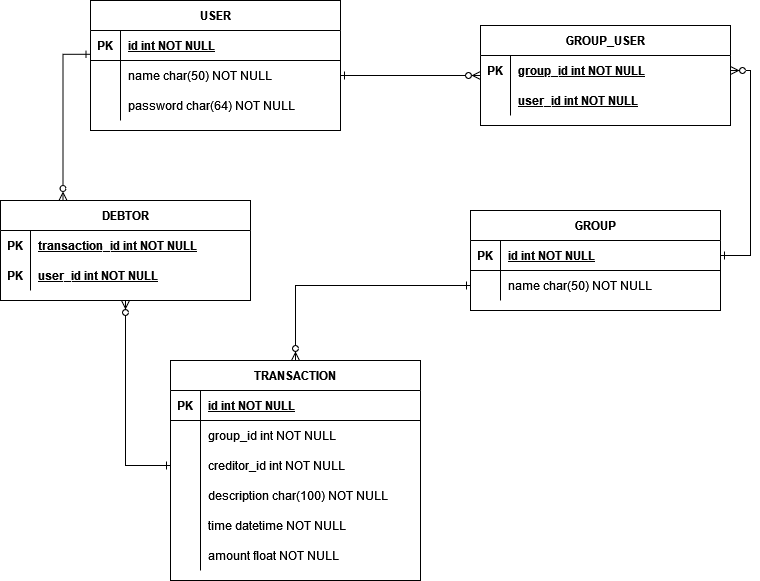
\includegraphics[width=\linewidth]{ER_Modell.png}
    \caption[Das ER-Modell der Datenbank]
    {Das ER-Modell der Datenbank}
    \label{fig:erModell}
\end{figure*}
Wie man im \gls{ER-Modell} (vgl. Abbildung~\ref{fig:erModell}) erkennen kann, gibt es fünf Tabellen.
\subsubsection{USER}
In dieser Tabelle wird der User bei der Registrierung angelegt. Gespeichert werden sein eingegebener Name, der nicht in der Datenbank vorhanden sein darf, sowie der \gls{Hash-Wert} seines Passworts.
Außerdem erhält er eine ID als primären Schlüssel.
\subsubsection{TRANSACTION}
Hier befinden sich die einzelnen Ausgaben. Eine Ausgabe enthält die ID der Gruppe, die ID des Gläubigers, eine Beschreibung, das Datum der Ausgabe, sowie einen Betrag.
\subsubsection{DEBTOR}
Um nun einem \gls{Schuldner} eine Ausgabe eines Gläubigers zuzuweisen, gibt es die Debtor-Tabelle.
Hier wird eine Ausgabe mit einem User verknüpft. So können zu einer Ausgabe mehere Schuldner zugewiesen werden.
\subsubsection{GROUP}
In der Group-Tabelle werden eine eindeutige ID, sowie der Name der Gruppe gespeichert.
\subsubsection{GROUP-USER}
Auch muss die Gruppenzugehörigkeit gespeichert werden. Hier finden sich die ID des Users mit der jeweiligen ID der Gruppe, in der er sich befindet.
So kann zugeordnet werden, welche User in welchen Gruppen ist.


\section{Randbedingungen}
Um mit der Entwicklung starten zu können, müssen vorher Bedingungen besprochen werden, welche von allen Mitgliedern eingehalten werden sollen.
So wird sichergestellt, dass das System auf jedem Rechner der Entwickler läuft und auch der Code ein einheitliches Erscheinungsbild hat.
\subsection{Technische Randbedingungen}
Als Entwicklungsumgebung wird VS Code verwendet.
Zudem gibt es Richtlinien für das Testen der Software:
\begin{itemize}
    \item Für jede Frontend-Komponente wird ein \gls{Unit-Test} mit \gls{Vitest} und dem React-Testing-Framework geschrieben.
    \item Für Backend-Endpunkte werden auch Unit-Tests mit Vitest und möglicherweise auch mit \gls{Postman}-Anwendung erstellt.
    \item Um die einzelnen Aktionen, die mit der Datenbank in Verbindung stehen, zu testen, werden die Tabellen (vgl. Abbildung~\ref{fig:erModell}) mit Testdaten gefüllt.
    \item Wichtig ist auch, dass Komponenten untereinander getestet werden. Das heißt, dass der Autor sein Werk nicht manuell selbst testet, da hier die Wahrscheinlichkeit, Fehler zu finden, geringer ist.
\end{itemize}
Außerdem wird MUI als Komponenten-Bibliothek für das Frontend verwendet, um kostbare Zeit beim Design zu sparen.
Falls Icons verwendet werden, werden die Material-Icons benutzt. Zu finden sind diese hier: \url{https://fonts.google.com/icons?selected=Material+Icons}.
\subsection{Organisatorische Randbedingungen}
Um einen reibungslosen Ablauf zu gewährleisten, wird jede Woche Montag im \gls{Weekly-Meeting} nach der Feedback-Session besprochen, was es an Aufgaben gibt und was in der kommenden Woche getan werden muss.
Anwesend sollten alle Mitglieder sein, sofern sie nicht durch Krankheit oder sonstige Notfälle verhindert sind.
Da es noch Personen im Team gibt, die weniger Erfahrung mit dem Framework React haben, werden \gls{Mentee}-\gls{Mentor}-Beziehungen gebildet, sodass es einen konkreten Ansprechpartner bei Problemen oder Fragen gibt.
Der Mentor ist dazu angehalten, sich bei Problemen um seinen Mentee zu kümmern.
Wo es möglich ist, sollte \gls{Peer-Programming} betrieben werden, da es zum Einen beim Lernen des Frameworks hilft und zum Anderen auch Austausch über mögliche alternative Lösungen stattfindet.
\subsection{Codier-Richtlinien}
Damit der Programm-Code ein einheitliches Bild abgibt, müssen Codier-Richtlinien eingehalten werden. Diese wurden von allen Gruppenmitgliedern erstellt.
Jedes Mitglied ist dazu angehalten, zu prüfen, ob folgende Richtlinien eingehalten wurden und gegebenenfalls Änderungen vorzunehmen, um die Einhaltung sicher zu stellen.
\begin{itemize}
    \item Format zur Benennung neuer \gls{Branches}: ,, \textlangle \gls{Issue}-Nummer\textrangle- \textlangle Name-des-Issues\textrangle''
    \item Die Format-Einstellungen für den Programm-Code sind in der Datei ,,prettierrc.json'' festgehalten und werden automatisch von der \gls{VS-Code}-Erweiterung ,,\gls{Prettier}'' genutzt und bei jedem Speichern umgesetzt.
    \item Der Programm-Code wird auf Englisch geschrieben.
    \item Die Sprache der Benutzeroberfläche ist allerdings auf Deutsch.
    \item Es sollten möglichst spezifische Typen verwendet werden, das heißt kein ,,any''.
    \item Keine Verwendung von ,,var''. Es sollten lieber ,,const'' oder ,,let'' benutzt werden.
    \item Funktionen-, sowie Variablennamen sollten ohne Kommentar in ihrer jeweiligen Funktionalität nachvollziehbar sein.
    \item Nur, wenn Funktionen- und Variablennamen nicht eindeutig auf die Funktionalität hindeuten, sollten Kommentare verwendet werden.
    \item Der Umfang einer Methode wird auf ein Minimum beschränkt, das heißt, so viel wie nötig und so wenig wie möglich.
    \item Methoden sollten nicht mehr machen, als ihr Name vermuten lässt.
    \item Methoden, Variablen und Ordnernamen werden in ,,\gls{camelCase}'' geschrieben.
    \item Für Typen, Klassen und React-Komponenten gilt hingegen ,,\gls{PascalCase}''.
\end{itemize}

%Vorbereitung für Tabelle
\renewcommand{\arraystretch}{2} % changes all rows to height 3
\newcolumntype{a}{>{\centering\arraybackslash}m{(\linewidth)/2}|}

\begin{center}
   \begin{table*}
    \centering
    \begin{NiceTabular}{|r||l|}
    \CodeBefore
        \rowcolors{1-1}{lightgray}{}
    \Body\Hline
    Architekturziel & Zugeordneter Architekturansatz        \\\Hline\Hline
    Im Backend sind keine anderen Programmierfähigkeiten als im Frontend notwendig.       & NodeJS                                       \\\Hline
    Während der Entwicklungszeit gibt es eine statische Typisierung.                      & TypeScript                                   \\\Hline
    REST-API weist geringen Implementierungsaufwand auf.                                  & Express.js                                   \\\Hline
    Die Daten werden in einer relationalen Datenbank gespeichert und bereitgestellt.      & MySQL                                        \\\Hline
    Der Zugriff auf die MySQL-Datenbank ist schnell, sicher und ohne SQL-Befehle möglich. & Sequelize                                    \\\Hline
    Die Webseite hat einen modularen Aufbau.                                              & React                                        \\\Hline
    Nutzer werden authentifiziert.                                                        & \gls{JWT} als Cookie im Frontend gespeichert \\\Hline
    Effizientes Kompilieren und \gls{Hot-Reloading} bei der Entwicklung des Frontends.    & Vite                                         \\\Hline
    Frontend und Backend werden automatisiert getestet.                                   & Vitest und Jest                              \\\Hline
    Stylesheets sind übersichlicher definiert.                                            & SCSS                                         \\\Hline
    Das Aussehen der Webseite ist einheitlich.                                            & Material UI                                  \\\Hline
    Die Entwicklung der Webseite ist zeitsparender.                                       & Material UI                                  \\\Hline
    Einheitliche Versionierung der Datenbank und Einspielen der Testdateien.              & Docker                                       \\\Hline
    Das Codeformat ist einheitlich.                                                       & Prettier                                     \\\Hline
    \end{NiceTabular}
    \vspace*{1em}

    \caption{Dem Architekturziel ist jeweils eine Technologie zugeordnet}
    \label{tab:loesungsstrategie}
  \end{table*}
\end{center}

\section{Ausblick}
Obwohl es sich bei ,,Wo ist mein Geld?'' um ein lauffähiges System handelt, bei dem alle geplanten User-Stories umgesetzt wurden, gibt es noch die Möglichkeit, weitere Features zu implementieren.
\begin{itemize}
    \item Gänzliche Optimierung der Anwendung für mobile Endgeräte
    \item Unterstützung mehrerer Sprachen
    \item Zusätzliche Informationen zu den Ausgaben, z. B. Bilder, Textbeschreibung, Schlagwörter, etc.
    \item Such- und Filterfunktion für Ausgaben
    \item Bearbeiten einer bestehenden Ausgabe
    \item Anzeige aller Gruppenmitglieder einer Gruppe
    \item Erstellen und Anzeigen einer Gruppenbeschreibung
    \item Bearbeiten des eigenen Nutzerprofils
\end{itemize}

\newpage
\printglossary[style=altlist,title=Glossar]
\vspace{12pt}

\end{document}
